\chapter{Prototype Implementation}
\label{chap:referenceimplementation}

As already discussed in chapter \ref{chap:introduction}, sensing a city's parking availability and thus making the parking situation more transparent would be highly beneficial for reducing traffic congestion and greenhouse gas emissions as driver's looking for parking spaces in urban areas could navigate directly to vacant parking spaces close to their destinations. In this thesis a prototype of drive-by sensing using an optical distance sensor was designed, implemented and evaluated.

This chapter will describe the setup and implementation of the prototype. In particular, section \ref{sec:system_design} will discuss the overall envisioned system, the prototype car and the required sensors with their capabilities. In section \ref{sec:experiment_description_data_collection} the experimental setup will be discussed as well as the acquiring of the test dataset through test drives in the city of Linz, Austria. Finally, section \ref{sec:data_processing} will describe the preprocessing of the data, definition of the features and a short description of all used machine learning algorithms with their configurations. \todo{update :)}

\section{System design}
\label{sec:system_design}

This section will describe the envisioned system for the urban parking availability detection system. The proposed system is a mobile sensing system where sensing vehicles try to detect parking cars while driving through the city. The sensing vehicles are equipped with several sensors. Most importantly an optical distance sensor measures the distance to the nearest obstacle on the right side of the road continuously while the vehicle is driving through the city. Furthermore, a GPS receiver determines the corresponding positions. 

- System description (type of sensors, requirements); overall envisioned system of cars detecting free spaces and communicating the information

\subsection{Test bed description}
\label{sec:test_bed}

- Testbed description (concrete HW and technical capabilities)

Figure \ref{fig:sensing_car} shows the sensing car and its mounted sensors. 

\begin{figure}
	\centering
	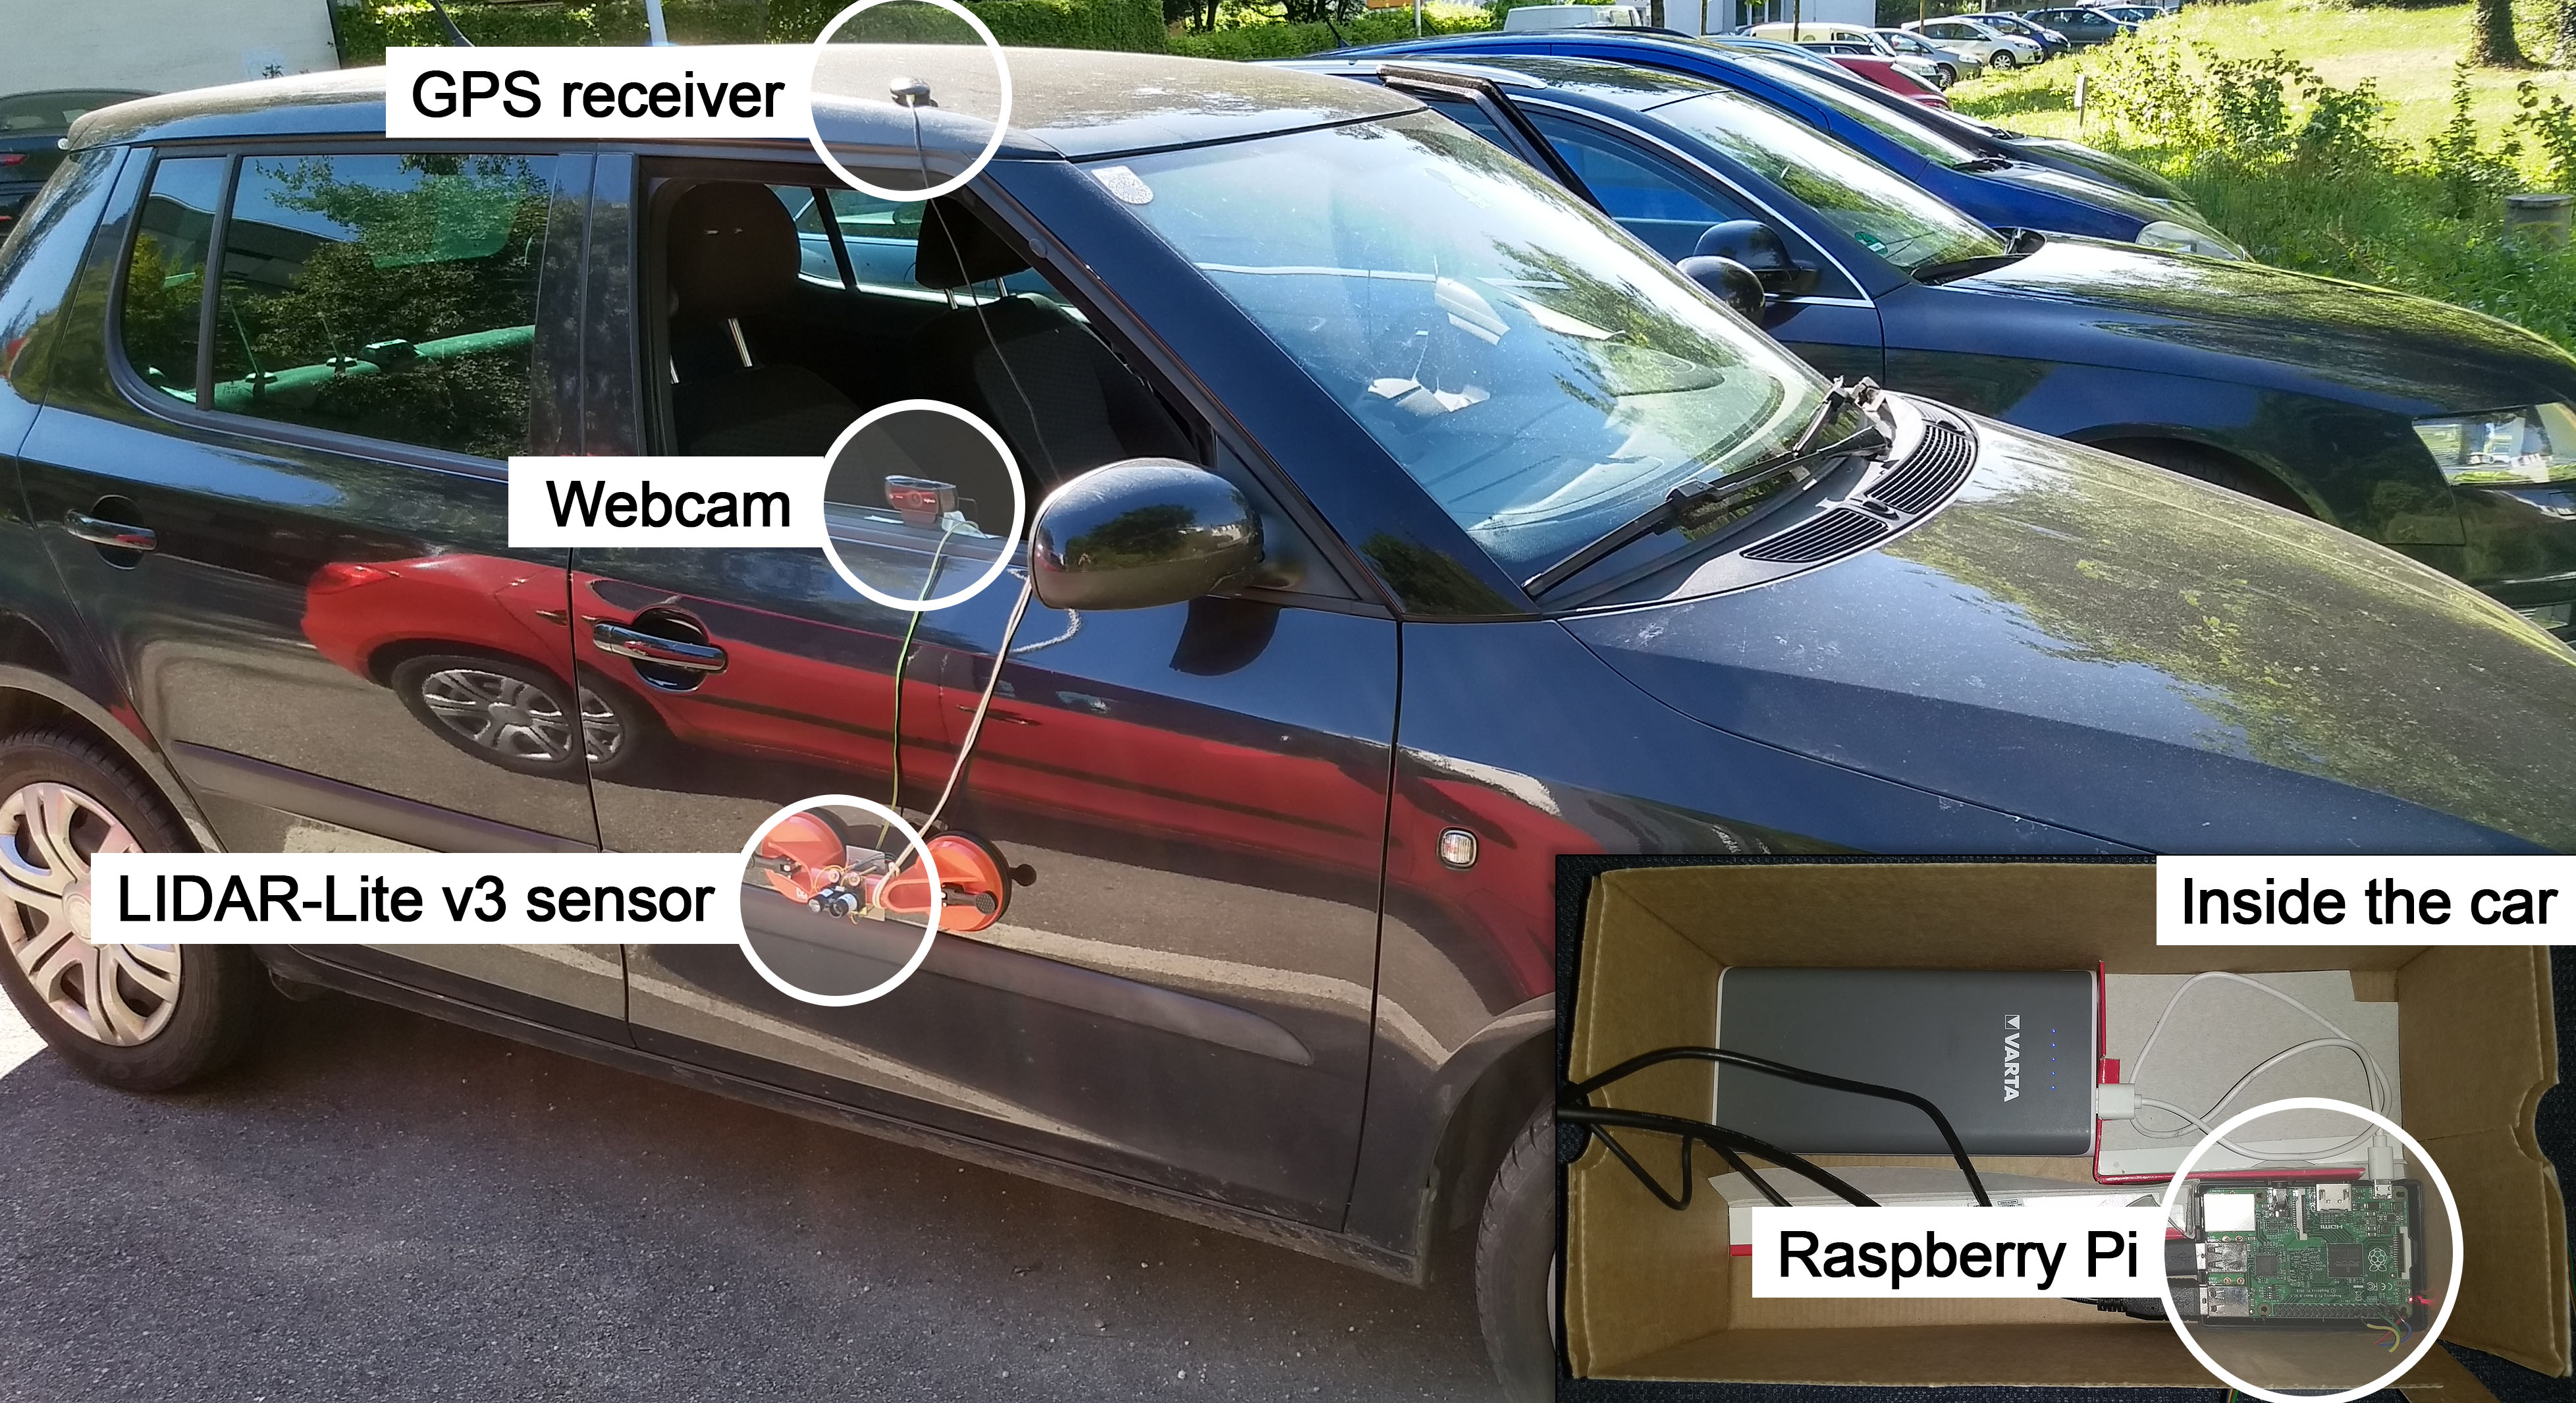
\includegraphics[width=\textwidth]{img/car.jpg}
	\caption{Prototype of the sensing car, which is composed of a LIDAR Lite v3 optical distance sensor, a GPS receiver, a camera for ground truth collection and a Raspberry Pi as processing device}
	\label{fig:sensing_car}
\end{figure}



\begin{table}

\bgroup
\def\arraystretch{1.5}
\begin{tabular}{| r || c | c |}
\hline
   & 
   \textbf{Sampling Frequency} & 
   \textbf{Costs per Sensor} \\
%\hline
\hline
  \textbf{Lidar Lite v3} & 
   ~200 measurements/s &
   \euro{169,00} \\
\hline
  \textbf{Navilock USB} & 
   ~1 measurement/s &
   \euro{74,90} \\
   \textbf{GPS receiver} & & \\
\hline

\end{tabular}
\egroup

\caption{The used sensors}
\label{table:sensors_capabilities}
\end{table}


\section{Experiment description and data collection}
\label{sec:experiment_description_data_collection}
- Description of experiments (scenarios we are interested in: parking car, etc.)
- Data set derived (raw data, size, etc.)
- Map data and camera ground truth data

\section{Data processing}
\label{sec:data_processing}
- Preprocessing, feature definition ...
- Traditional ML Algorithms (incl. a short description of each algorithm and configuration options)
- Deep Learning

\section{Experimental results}
- Results of the different ML approaches, important features, difficult cases, etc.
- Comparison of traditional ML and Deep Learning (cf. our demo)